\chapter{Graphes de tâches}
%
\newcommand{\RR}{\mathbb{R}}
\newcommand{\forto}{\text{\bf\ to\ }}
\newenvironment{defi}[1][Definition]{\begin{trivlist}
\item[\hskip \labelsep {\bfseries #1}]}{\end{trivlist}}
%
Dans ce chapitre, nous introduisons les concepts concernant la description des applica-tions parallèles à base de tâches en particulier les graphes de tâches, le modèle DAG et les modèles d'ordonnancement. Son objectif est de présenter les particularités structurelles de cette classe d'applications ainsi que son aspect fonctionnel lors de son ordonnancement et son exécution sur une plateforme multiprocesseurs.  

%Application parallèle décrite par DAG
Dans la section \ref{secAPdpDAG}, nous décrivons tout d’abord les applications à base de tâches ainsi que le graphe de tâches comme outils pour cette description.
%Modèle DAG
Ensuite dans la section \ref{modelDAG}, nous considérons le modèle DAG et nous présentons les concepts et la terminologie qui ont relation avec ce type de graphe. L'aspect dynamique résultant de son exécution sur une plateforme parallèle sera décrit en détail dans cette section.   
%Modèle d'ordonnancement
Les modèles d'ordonnancement ainsi que les algorithmes de résolution sont présentés dans la section \ref{modelSched}.
%Conclusion
Enfin la section \ref{concDAG} conclue ce chapitre.
%======================================================================================================
\section{Application parallèle décrite par DAG}\label{secAPdpDAG}
%
La parallélisation efficace d'une application nécessite une connaissance approfondie de la structure du programme. 
Il existe plusieurs méthodes pour déclarer la structure parallèle du programme à partir de sa version séquentielle en spécifiant les blocs (sections) séquentiels et leurs relations, souvent faite manuellement par le programmeur, 
Ces métho-des sont appelées les \textbf{modèles de la programmation parallèle}.
Comme exemples de ces modèles, on peut citer 
Fork-Join pattern \cite{ABB00}, les 
MPI (passage de messages) \cite{GLS99}, 
map-reduce pattern \cite{DG04}.
Ces modèles diffèrent dans leur API, dans leur granularité et leur fonctionnalité, 
ils partagent tous un objectif commun : 
partitionner le programme séquentiel et 
exécuter les blocs séquentiels résultants dans un ordre qui préserve leurs dépendances mutuelles sur la plateforme parallèle cible sur laquelle on exécute l'application (appelé \textbf{environnement d'exécution}).
La deuxième partie de ce processus (trouver cet ordre) s'appelle l'\textbf{ordonnancement}. 
Les blocs séquentiels représen-tent des parties du code séquentiel du programme sont appelés les \textbf{tâches}. 
L'environnement d'exécution matériel et logiciel où un algorithme ou l'application parallèle s'exécutent est appelé le \textbf{modèle de système}.
%
\subsection{Graphe de tâches}\label{ullmanNP}
%
Les dépendances entre les tâches représentent la relation fonctionnelle causale ou un partage de ressources ou de données (qui nécessitent d'être placées et transferées) entre les tâches concernées. Les données  utilisées par les tâches précédentes après leurs exécutions doivent être mises à jour et préparées pour les tâches suivantes. 
Ces relations de dépendance entre les tâches peuvent être modélisées en tant que graphe, et donc toutes les dépendances représentent une causalité de précédence temporelle ce qui empêche l'existence de tout cycle dans ce graphe (retour vers des tâches déjà exécutées) 
Ainsi, ce modèle s'appelle \textbf{Graphe acyclique dirigé (DAG)}.
%
%\begin{figure}
%\includegraphics[scale=0.75]{dag010}
%\centering
%\caption{Exemple d'une application parallèle décrite par un DAG}
%\label{fig:FG_3_1}
%\end{figure} 
%
%La figure \ref{fig:FG_3_1} montre un exemple d'un DAG qui modélise un programme parallèle. 
%
\begin{figure}
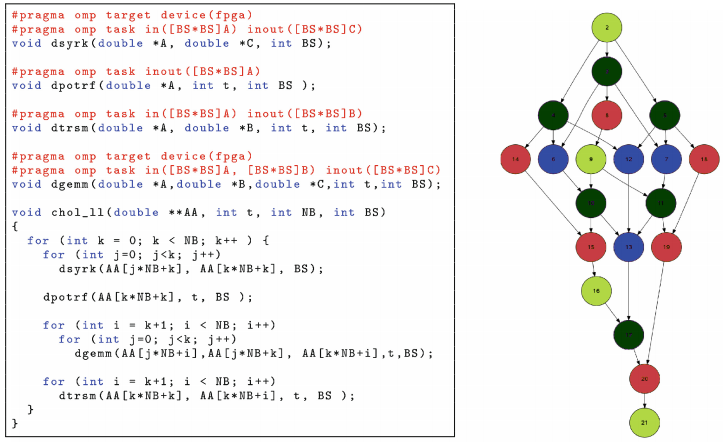
\includegraphics[scale=0.75]{dag011}
\centering
\caption{Exemple d'un code OpenMP parallèle et son DAG équivalent}
\label{fig:FG_3_1_0}
\end{figure} 
La figure \ref{fig:FG_3_1_0} montre un exemple d'un code OpenMP parallèle et son DAG équivalent.
%
Le problème de l'ordonnancement des programmes parallèles décrits par un DAG consiste à trouver l'ordre d'exécution (ressources temporelles) des tâches constituantes le programmes et sa projection sur la plateforme parallèle (ressources spatiales) de façon consistante qui respecte le principe de la causalité.
\textbf{Ullmann et al} ont montré que le \textbf{problème de l'ordonnancement d'un DAG sur une machine multiprocesseur} est un \textbf{problème NP-complet} sous sa forme générale \cite{Ull75}.
%
Les techniques d'ordonnancement les plus populaires ne tentent pas de trouver nécessairement un ordre optimal. 
Au lieu de cela, ils tentent d'en trouver un qui respecte leurs dépendances mutuelles et est en corrélation avec une métrique d'importance spécifiée qui favorise les tâches les plus importantes et les plus critiques pour l'exécution globale de l'application \cite{KA99}. 
La tâche de l'ordonnanceur ne dépend pas seulement de l'application parallèle à ordonnancer mais aussi de l'environnement de l'exécution.
%
Les techniques d'ordonnancement (algorithmes, politiques, stratégies) se caractérisent par la quantité d'informations et les détails à-propos du DAG exploitées pour réaliser son objectif.
Certains algorithmes utilisent peu d'informations sur la structure du programme dans ce processus 
(Certes une connaissance plus complète de la structure du programme, sa prise de décision peut devenir plus raisonnable et plus efficace, 
Mais en réalité beaucoup de ces informations ne sont pas disponibles lors de la conception (désigne-time) mais au moment d'exécution du programme (runtime)),  
Au lieu de cela, ils essaient d'utiliser des modèles qui donnent à un ordonnanceur une connaissance restreinte de la structure du programme lui permettant d'améliorer les performances dans un environnement d'exécution donné ce qui les rend plus rapides (atteindre une meilleure performance en ne connaissant qu'une partie de la structure du programme) \cite{HL14}.

Les propriétés de l'environnement où l'ordonnanceur agit ont une influence majeure sur la structure de l'algorithme d’ordonnancement. 
Selon que les processeurs soient ou non homogènes, quelle est la topologie de la plateforme, les informations sur le programme, etc., l'algorithme peut prendre ses décisions en considérant des informations très différentes. 
L'aspect principal est de savoir comment les propriétés de l'ordonnancement résultant dépendent de l'exhaustivité des informations disponibles pour l'algorithme. Le modèle de système se compose de trois composants : \\
%
- modèle plateforme\\
- modèle interconnexion\\
- modèle ordonnancement 

- \textbf{Le modèle plateforme} : décrit les propriétés des plateformes (processeurs, nœud de calcul,  ..), qui exécutent un programme parallèle et l’ordonnanceur lui-même. 
Les processeurs d'une plateforme peuvent être homogènes ou hétérogènes. 

- \textbf{Le modèle interconnexion} : décrit les propriétés des liens de communication qui connectent les processeurs et leur topologie.
Les liens de communication peuvent être une ressource partagée qui nécessitent une concurrence pour l'utiliser alors il faut gérer le conflit de ce partage dans ce contexte (avec conflit with-contention) ou être sans contention (contention-free). 
%
(Contestation-free, une fois qu'une opération de communication démarre, elle ne subit aucune perturbation par rapport à d'autres opérations de communication,
Cela signifie qu'une opération de communication occupe exclusivement le canal entre les deux processeurs et ne peut pas être interrompue). 

- \textbf{Le modèle ordonnancement} : décrit les informations disponibles pour un ordonnan-ceur et la manière dont son algorithme peut fonctionner avec ces informations disponibles.

Les algorithmes manipulant les graphes de tâche et générant les ordonnancement correspondants à une application décrite par ce modèle peuvent être divisés en deux classes suivantes :

1- \textbf{Algorithmes just-in-time (JIT-algorithmes)} 

Ces algorithmes ont très peu d'informations sur le programme pour lequel ils tentent de trouver un ordre d'exécution. 
Leurs décisions sont prises en runtime. 
Et la minimisation des coûts d'ordonnancement est souvent un objectif important pour eux. 

2- \textbf{Algorithmes complets}

Ces algorithmes connaissent la structure complexe du programme. %
Ils font chaque décision d'ordonnancement en tenant compte des répercussions possibles de l'avenir. 
Tout cela permet de réaliser toutes les actions nécessaires avant l'exécution de l'application, en temps de compilation (design-time). 
%===========================================================================
\section{Modèle DAG} \label{modelDAG}
%
L'exécution de programme parallèle se compose des tâches (code séquentiel), qui ont des dépendances de données entre elles. 
Une telle structure peut être modélisée selon un graphe dirigé acyclique (DAG), où 
les nœuds représentent des tâches (parties séquentielles) et 
des arcs (arêtes) représentent des dépendances de données. 
Divers paramè-tres du programme peuvent être modélisés soit comme attributs des nœuds, des arcs ou du graphe lui-même. 
%
\subsection{Concepts et définitions} 
%
Afin de montrer le processus de la description d'un code parallèle par un DAG, nous allons définir les concepts de base pour cette transformation et les notations utilisées par la suite. 
Nous commençons par la présentation d'un exemple de code séquentiel d'algorithme pour un problème classique du calcule numérique 'résolution d'un système d'équations dont la matrice est triangulaire' qui va servir de modèle.
  
Soit le problème de la résolution d'un système d'équation suivant : $A\cdot x=b$ \\
\begin{itemize}
    \item $A \in MTI_n(\RR)$ Matrice triangulaire inferieure donnée
    \item $b \in\RR^n$ vecteur constant
\end{itemize}

L'algorithme $AL001$ suivant calcule la solution de ce système :
%
\begin{algorithm}
  \caption{Résolution systeme d'équations}
  \DontPrintSemicolon
  \For{$i=1 \forto n$}{
	Task $T_{i,i}: x_i \gets \frac{b_i}{a_{i,i}}$\;
	\For{$j=i+1 \forto n$}{
	  Task $T_{i,j}: b_j \gets b_j - a_{i,j}x_i$
	}
  }
\end{algorithm}
%
Cet algorithme est séquentiel, la totalité du calcule est faite par les blocs de code (Tâche $T_{ij}$) de l'algorithme ou l'exécution de ces blocs suit un ordre total définit par la structure séquentielle du code.
%
\begin{définition}[Calculer Avant $<_{seq}$.]\textit{
%
On définit la relation d'\textbf{ordre total} sur $AL001$ \textbf{calculer avant} $<_{seq}$ :  
$$
T <_{seq} T'   \implies T \text{ est calculée / exécutée avant } T'
$$
%
}\end{définition}
%
On a l'ordre suivant pour les tâches de $AL001$ : $T_{1,1} <_{seq} T_{1,2} <_{seq} T_{1,3} <_{seq} \dots <_{seq} T_{1,n} <_{seq} T_{2,2} <_{seq} \dots <_{seq} T_{n,n}$

La logique de l'exécution des $T_{i,j}$ est la suivante : \\
- $T_{1,1}$ est la première tâche et calcule $x_1$, \\
- $T_{1,2}$ et $T_{1,3}$ utilisent $x_1$, elle doit attendre la fin de $T_{1,1}$ (calcul de $x_1$).\\
- $T_{1,2}$ met à jour $b_2$ et $T_{1;,3}$ met à jour $b_3$. $T_{1,2}$ et $T_{1,3}$ sont indépendantes et peuvent être exécutées dans n'importe quel ordre.

On caractérise la Tâche $T$ par :\\
- $In(T)$    : l'ensemble des variables lues par la tâche $T$.\\
- $Out(T)$  : l'ensemble des variables écrites par la tâche $T$.
%
\begin{définition}[Variables partagées.]\textit{
%
On définit l'ensemble $SV$ des \textbf{variables partagées} entre $T$ et $T'$ l'ensemble des variables qui peuvent être modifiées par les deux tâches ou une des tâches et lues par l'autre au cours de l'exécution. 
$$
SV(T,T') = ((Out(T) \cap Out(T')) \cup (Out(T) \cap In(T')) \cup (Out(T') \cap In(T))
$$
%
}\end{définition}
%
\begin{définition}[\textsc{Bernstein} conditions.]\textit{
%
$T$ et $T'$ sont \textbf{dépendantes}, si et seulement si elles partagent certaines variables à modifier $T \bot T'$.
%
$$
T \bot T' \iff SV(T,T') \neq \emptyset
$$
%
}\end{définition}
%\textbf{\textsc{Bernstein} conditions}
Dans l'exemple donné, on a $Out(T_{1,1}) \cap In(T_{1,2}) = \{x_1\}$ alors $T_{1,1} \bot T_{1,2}$ et $Out(T_{1,3}) \cap Out(T_{2,3}) = \{b_3\}$ alors $T_{1,3} \bot T_{2,3}$.

Si $T \bot T'$ alors elles doivent être ordonnées selon l'ordre de l'exécution séquentielle.
%
\begin{définition}[Relation de Précédence $\prec$.]\textit{
%
$T$ précède $T'$ si et seulement que $T$ et $T'$ partagent certaines variables et $T$ doit être exécuter avant $T'$ $T \prec T'$.
%
$$
T \prec T' \iff (T \bot T') \& T \leq_{seq} T'
$$
%
}\end{définition}
%Alors on a $T \prec T'$ $ \prec:= (<_{seq} \cap \bot)^+$
$\prec$: est un \textbf{ordre partial} (consistant avec $<_{seq}$): $< = (<_{seq} \cap \bot)^+$

Dans l'exemple, on a : 
$T_{2,4}$ et $T_{4,4}$: $T_{2,4}$ modifie $b_4$ et $T_{4,4}$ lit $b_4 \implies T_{2,4} \bot T_{4,4}; T_{2,3} < T_{4,4}$

$T_{4,4}$ et $T_{4,5}$: $T_{4,4}$ modifie $x_4$ et $T_{4,(}$ modifie $x_4 \implies T_{4,4} \bot T_{4,5}; T_{4,4} < T_{4,5}$

$T_{2,4}$ et $T_{4,5}$: $T_{2,4}$ et $T_{4,5}$ sont indépendantes 

\paragraph{Représentation par un graphe dirigé}
$G = (V,E)$\\
$V$ = ensemble de tâches.\\
$e=(T,T') \in E \iff T < T'$ relation de précédence $T$ est prédécesseur de $T'$
%
\begin{figure}  %[h]
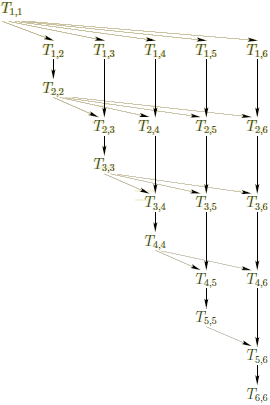
\includegraphics[scale=0.75]{dag006}
\centering
\caption{DAG de l'application résolution d'un système d'équations \cite{Dreb15}}
\label{fig:FG_3_2}
\end{figure} 
%
La figure \ref{fig:FG_3_2} montre le DAG correspondant au programme donné en exemple. 

Cette représentation donne un graphe dirigé et sans cycle appelé \textbf{graphe de précéden-ce} ou de \textbf{tâches  (DAG direct acyclic graph)} dont les nœuds sont des tâches (\textbf{calcul}) et les arcs représentent les dépendances entre les tâches (\textbf{communication}). 
Souvent cette description peut être complétée par les informations d'exécution (la durée de chaque tâche $w$, le volume des données échangées entre deux tâches communicantes $c$ si elles sont disponibles) dans certains cas DAG(T, <, w, c). 
Le coût de ce calcul et de cette communication ne dépend pas seulement de la durée des tâches et du volume échangé entre les tâches communicantes mais aussi des caractéristiques la plateforme sur laquelle elles s'exécutent.
C'est pourquoi il est important de caractériser et modéliser cette plateforme pour quantifier correctement les performances des politiques gérant l'exécution des applica-tions parallèles sur ces plateformes. La modélisation la plus simple est de représenter l'architecture cible par l'ensemble de ressources d'exécution (processeurs, cœurs, nœuds, ou autre) $\mathbb{P} = \{P_i\}_{i \in I}$ en donnant leurs caractéristiques.

Par la suite on va utiliser les fonctions suivantes :\\
- $\delta_\triangleleft(v_i)$ : \textbf{fonction prédécesseur} renvoie une liste des tâches qui précèdent la tâche $v_i$ (les tâches mères (nœuds parents prédécesseurs)).\\
- $\delta_\triangleright(v_i)$  : \textbf{fonction successeur} renvoie une liste des tâches dont l'exécution dépend de la tâche (du nœud) $v_i$ (tâches filles (successeurs)).\\
- $w(v_i)$ : \textbf{coût de calcul du travail} $v_i$.\\
- $c(e_{ij})$ : \textbf{coût de communication} $e_{ij}$ le volume des données échangées entre deux tâches.

Si les tâches $v_i$ et $v_j$ sont programmées pour le même processeur, alors $c(e_{ij}) = 0$. 
Sans perte de généralité, supposons qu'un DAG ait un seul nœud d'entrée et qu'un seul nœud de sortie. 
Tous les nœuds, à l'exception des nœuds d'entrée et de sortie, (initiaux et terminaux) ont des poids positifs $w(v_i) > 0$. 

Le \textbf{niveau statique sl} d'un nœud $v_i$ est la longueur du chemin le plus long du nœud $v_i$ au nœud de sortie, y compris le poids de $v_i$. 
S-level ne considère pas les coûts de communication, donc il ne dépend pas d'un ordonnancement particulier. 
%
$$
sl(v_i) = if(\delta_\triangleright(v_i) = \varnothing , 0 , \max_{ v_j \in \delta_\triangleright(v_i)}\{ sl(v_j) \} + w(v_i)
$$
%
Le \textbf{niveau statique supérieur (top) stl} d'un nœud $v_i$ est la longueur du chemin le plus long du nœud d'entrée vers un nœud $v_i$, à l'exclusion du poids de $v_i$. 
Le niveau statique supérieur inclut tous les coûts de communication et calculé avant l'établissement de l'ordonnancement. 
Ainsi, le calcul à un niveau ne considère pas la possibilité d'annuler les coûts de communication, lorsque des tâches dépendantes s'exécutent sur le même processeur. 
%
$$
stl(v_i) = if(\delta_\triangleleft(v_i) = \varnothing , 0 , \max_{ v_j \in \delta_\triangleleft(v_i)}\{ stl(v_j) + w(e_{ji})  + w(v_j) \}
$$
%
Le \textbf{niveau statique inférieur (bottom) sbl} d'un nœud $v_i$ est la longueur du chemin le plus long du nœud $v_i$ au nœud de sortie, y compris le poids de $v_i$. 
Le calcul du niveau b statique inclut les coûts de communication de la même manière qu'avec le niveau t. 
%
$$
sbl(v_i) = if(\delta_\triangleright(v_i) = \varnothing , 0 , \max_{ v_j \in \delta_\triangleright(v_i)}\{ sbl(v_j) + w(e_{ij}) \} + w(v_i)
$$
%
Le \textbf{travail total (W)} est la poids totale de toutes les tâches dans le DAG. 
Si toutes les tâches sont programmées sur le même processeur, la durée de l'ordonnancement résultant est égale au travail total. 
La formule pour calculer le travail total est la suivante :
%
$$
W = \sum_{ v_i \in V} w(v_i)
$$
%
Le \textbf{chemin critique (CP)} désigne la longueur du chemin le plus long du nœud d'entrée au nœud de sortie. 
Un DAG peut avoir plusieurs chemins critiques de même longueur. 
La longueur de chemin critique équivaut au niveau s d'un nœud d'entrée. 
Le chemin critique est un paramètre important d'un DAG, car il montre la limite inférieure de toute longueur de programme possible : 
Même avec une quantité illimitée d'exécution de processeurs ne peut pas prendre moins que l'exécution du chemin critique requiert. 
Le chemin critique peut également inclure les coûts de communication existant entre les nœuds dans le chemin critique. 

Les paramètres mentionnés ci-dessus ne dépendent pas d'un ordonnancement particulier qui peut affecter des tâches aux processeurs de manière différente. 
Ces paramèt-res sont appelés statiques. 
%
\subsection{Exécution  d'un DAG}  %3.1
%
Soit le DAG $G(V,E,w,c)$ qui décrit la structure d'une application parallèle que nous allons l'exécuter sur la plateforme de $m$ processeurs  $\mathbb{P} = \{P_i\}_{i \in [1..m]}$
%
\begin{définition}[Principe de causalité.]\textit{
%
L'ordonnancement d'un DAG $G(V,E,w,c)$ est la fonction $\theta$ qui associe à  chaque tâche sa \textbf{date début} : 
\begin{align*}
  \theta \colon V & \to \mathbb{R}\\
  v_i                    & \mapsto s_i = \theta(v_i).
\end{align*}
%
Vérifiant la relation (\textbf{principe de causalité}) :  
$$\forall (v_i, v_j) \in E, \theta(v_i) + w(v_i) < \theta(v_j)$$
%
}\end{définition}
%
Apres avoir déterminé un ordre chronologique de l'exécution des tâches d'un DAG, nous allons définir une fonction qui assure la projection des tâches sur les processeurs de la plateforme cible.
%
\begin{définition}[Principe de non chevauchement]\textit{
%
L'allocation d'un processeur à une tâche d'un DAG est la fonction $\pi$ qui associe à  chaque tâche un processeur sur lequel elle va être exécuté (renvoie un \textbf{processeur alloué} à la tâche $v_i$) : 
\begin{align*}
  \pi \colon V & \to \mathbb{P}\\
  v_i                    & \mapsto p_j = \pi(v_i).
\end{align*}
%
Vérifiant la relation (\textbf{principe de non chevauchement}) : 
$$\forall (v_i, v_j) \in V^2, \pi(v_i) = \pi(v_j) \equiv (\theta(v_i)+ w(v_i) < \theta(v_j)) or (\theta(v_j)+ w(v_j) < \theta(v_i))$$
%
}\end{définition}
%
Un \textbf{algorithme d'ordonnancement} détermine le début d'exécution et le processeur alloué d'une tâche. 

En donnant un ordonnancement particulier $\theta_k$, on peut déterminer les paramètres dynamiques suivants :

Le \textbf{temps de début} d'une tâche dans un ordonnancement particulier est désigné par $ ST(v_i) =  s_i $.

Le \textbf{temps de la fin} d'une tâche dans un ordonnancement particulier est désignée comme $ ET (v_i) = e_i $. 
Entre le début et la fin d'une tâche, on la relation suivante :  
%
$$
ET(v_i) = ST(v_i) + w(v_i)
$$
%
Le \textbf{temps total d'exécution (completion time, Makespan)} indique le temps de fin de la tâche de sortie. Aussi appelée durée de l'ordonnancement. note $C_{max}(\mathcal{O}_k)$

Le \textbf{niveau dynamique supérieur top} d'une tâche $v_i$ sur un processeur $P_j$ est la longueur du chemin le plus long de la tâche d'entrée vers la tâche $v_i$, à l'exclusion du poids de $v_i$. 
Ce niveau indique le temps de début le plus tôt possible d'une tâche $v_i$, lorsque les tâches antécédentes de $v_i$ est déjà ordonnancées.
%
$$
tl(v_i) = if(\delta_\triangleleft(v_i) = \varnothing , 0 , \max_{ v_j \in \delta_\triangleleft(v_i)}\{ FT(v_j) + w(e_{ji}) \}
$$
%
Le niveau t dynamique ne considère pas la disponibilité d'un processeur prêt pour exécution du nœud vi, donc le temps réel le plus tôt possible peut être plus grand.

Le \textbf{niveau dynamique inférieur bottom} d'une tâche $v_i$ sur un processeur $p_j$ est la longueur du chemin le plus long de $v_i$ à la sortie, y compris le poids de $v_i$. Ce niveau est calculé comme suit.
%
$$
bl(v_i) = if(\delta_\triangleright(v_i) = \varnothing , 0 , \max_{ v_j \in \delta_\triangleright(v_i)}\{ bl(v_j) + w(e_{ij}) \} + w(v_i)
$$
%
Le \textbf{temps prêt $RT(v_i, p_j)$} est le temps le plus tôt possible lorsque le processeur $p_j$ peut exécuter la tâche $v_i$. 

Le \textbf{temps début au plus tôt $EST(v_i,p_j)$} fait référence au temps d'exécution le plus tôt possible de la tâche $v_i$ sur un processeur $p_j$. 
%
$$
EST(v_i, p_j) = max \{ tl(v_i) , R(v_i, p_j) \}
$$
%
Le \textbf{premier temps de finition $EFT (v_i; p_j)$} se rapporte au temps de finition le plus tôt possible d'un nœud $v_i$ sur un processeur $p_j$. Entre EST et EFT suivant relation tient.
%
$$
EFT(v_i, p_j) = EST(v_i , p_j) + w(v_i)
$$
%
Le \textbf{temps de la fin réelle (AFT)} est le moment où la tâche achève son travail dans un ordonnancement particulier. 

Le \textbf{Temps début au plus tard (ALAP)} est une métrique qui indique combien le début d'une tâche peut être retardé sans augmenter le makespan. L'ALAP des tâches du chemin critique est égal à leur niveau t.

En donnant un $DAG$ et un environnement d'exécution $ENV$ et $\mathbb{O}$ soit l'ensemble de tous les ordonnancements possible de DAG sur $ENV$.

Un \textbf{problème d'ordonnancement $\Pi_{( \mathcal{O} | DAG, ENV)}$} consiste à déterminer l'\textbf{ordon-nancement optimal $\mathcal{O}^*$} de l'exécution de DAG sur ENV dont $C_{max}$ est le minimum.
%
$$
\mathcal{O}^* = arg \min_{ \mathcal{O}_i \in \mathbb{O}} \{  C_{max}(\mathcal{O}_i())   \} 
$$
%
Comme nous avons cité dans la section \ref{ullmanNP}, que \textbf{Ullmann et al} ont montré que le \textbf{problème de l'ordonnancement d'un DAG sur une machine multiprocesseur} est un \textbf{problème NP-complet} sous sa forme générale \cite{Ull75}. Trouver $\mathcal{O}^*$ généralement n'est assez facile. C'est pourquoi on cherche une bonne solution qui proche à la solution optimale avec un coût acceptable.
%---------------------------------------------------------------------------
Le listing suivant donne le contenu du ficher random000.stg selon le format StandardTaskGraph (STG) d'un DAG générique de 50 tâches et les figures suivantes \ref{fig:FG_3_1002} montre son ordonnancement sur les plateformes UMA de 4 cœurs et 8 cœurs respectivement.
%
\begin{Verbatim}[formatcom=\color{blue}]
#StandardTaskGraphSetProject
#RandomTaskGraph50//tmp/50/rand0000.stg
   50
   0   0   0
   1   9   1   0
   2   4   1   0
   3   3   1   0
   4   6   1   0
   5   4   1   1
   6   3   1   5
   7   3   1   0
   8   8   1   6
   9   9   1   0
   10    2   3   2   6   8
   11    1   1   9
   .............
   48   2   5   23   28   29   40   41
   49   9   4   30   39   46   47
   50   10   3    20   32   46
   51   0   11   3   17   31   34   38   42   43   45   48   49   50
\end{Verbatim}
%
\begin{figure}
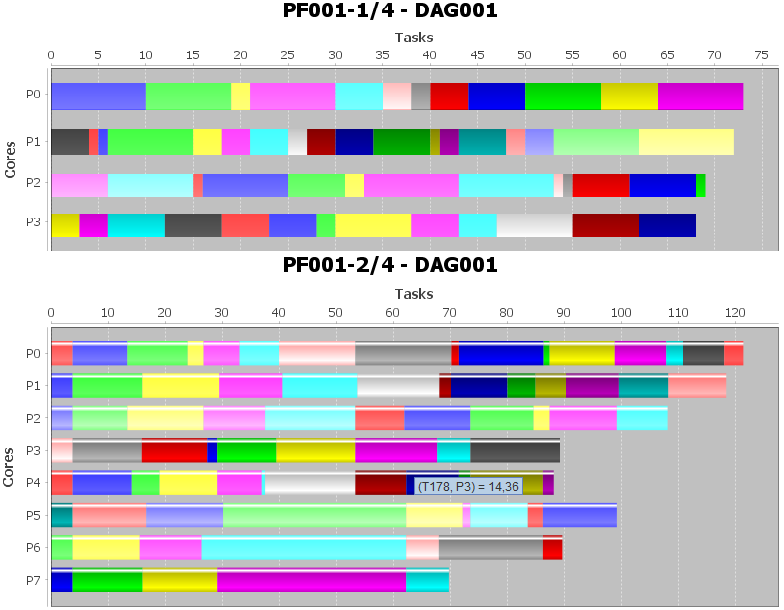
\includegraphics[scale=0.75]{dag10021}
\centering
\caption{Ordonnancement du DAG rand0000.stg sur des plateformes UMAs}
\label{fig:FG_3_1002}
\end{figure}
%===============================================================================
\newpage
\section{Modèle d'ordonnancement} \label{modelSched} 
%
Le modèle du système détermine la variété des algorithmes qui peuvent être utilisés. 
L'applicabilité du modèle est déterminée par les propriétés requises de l'environne-ment d'exécution. 
Des facteurs tels que les garanties de performance, la robustesse, la fiabilité et d'autres déterminent un modèle de système optimal et un algorithme d'ordonnancement optimal. 
Cette section présente des principes généraux d'ordonnancem-ent et des paradig-mes dans les modèles de système.
%
\subsection{Modèle Just-in-Time JIT}  
%
Le modèle Just-in-Time (JIT) ne prend pas en compte la structure du programme. 
Les ordonnanceur de ce modèle ne peuvent se permettre aucun ordre statique. 
On suppose qu'à chaque moment, un ordonnanceur connaît des informations très restreintes, mais cette information est à jour. 
Pour cette raison, les décisions de l'ordonnanceur doivent être prises immédiatement avant leur mise en œuvre, 

Dans le modèle just-in-time, les algorithmes d'ordonnancement des tâches DAG apparai-ssent pour l'ordonnanceur uniquement lorsqu’elles sont prêtes, i. e. toutes leurs dépendances sont satisfaites. 
Une tâche qui est en cours d'exécution sur un processeur est dite active. 
Si l'exécution d'une tâche dépend d'une autre tâche, alors la premiere est appelée une tâche-fille de la deuxième la tâche mère. 

Une queue globale et unique qui représente la file d'attente de tâches prêtes (dont l'état est prêt) est utilisée dans ce modèle. La tâche prête qui est en  entête de cette queue est affectée au processeur qui devient libre. 

Dans ce contexte, la contention pour le bus système peut diminuer drastiquement la latence et le débit du système \cite{ALL89} d'une part. 
D'autre part, L'influence de la localité des données sur le nombre de pertes de mémoire cache CPU \cite{HL14} et les défauts de page \cite{BLU96} participent à aggraver la situation. 
Cela augmente le trafic et la contenance du bus mémoire partagé et entraîne des pénalités de performance significatives. 

Si les tâches filles restent sur le même processeur que les tâches-mères, les pénalités de performance se développent plus lentement avec un nombre accru de processeurs \cite{SL93}.

\subsection{Horizon d'exécution pour les multicoeurs \cite{Pla15}}
L'ordonnancement est effectué en planifiant les tâches sur les processeurs disponib-les dans un ordre qui respecte les dépendances de données du DAG. 
%
Puisque initialement juste une information partielle sur l'application est disponible au support d'exécution, alors La prise de décision  se fait seulement au moment d'exécution de façon dynamique. 
Lorsqu'une application démarre, l'ordonnanceur découvre un certain nombre de tâches, à une certaine profondeur en fonction des tâches déjà traitées (soit complète, en exécution ou prête) ce qui constitue l'horizon d'exécution vu par l'ordonnanceur à ce moment. 
Certaines tâches sont prêtes à être exécutées juste après la fin de certaines tâches en exécution. Une fois qu'une tâche finit, l'ordonnanceur découvre ses descendants à une certaine profondeur et mis à jour l'horizon courant. Dans cet aspect, le modèle d'horizon est similaire au modèle JIT. Mais contrairement à ce dernier, l'ordonnanceur dans le modèle de l'horizon découvre plus d'informations après chaque étape d'exécution. Plus d'informations sur la structure de programme parallèle permettent à l’ordonnanceur qui permet de prendre une meilleure décision d'ordonnancement à chaque étape de l'exécution. 

Pour rendre cette information disponible, l'ordonnanceur peut utiliser les outils d'analy-se de code statique initialement pour extraction de certain aspect statique de l'application (sa structure, nombre des tâches,...) comme il peut utiliser les outils d'instru-mentation de l'exécution pour collecter les statistiques et les valeurs de certains paramètres après chaque événement d'exécution (la fin/début d'exécution d'une tâche, communication).

Les outils d'analyse de code statique devraient pouvoir reconnaître la structure de l'application (les parties séquentielles du programme et les dépendances entre eux). 
Le programmeur peut fournir certaines indications à ces outils en annotant le code source avec des directives dont l'interprétation par le compilateur permet de renseigner le support exécutif de certaines détails. 
En outre, l'outil d'analyse de code statique devrait pouvoir annoter l'image binaire du programme avec les informations sur ces parties séquentielles. 
Ces annotations devraient être reconnues par une partie dynamique d'un système parallèle, qui fournit un ordonnanceur avec une connaissance de l'horizon.
%
L'ordon-nanceur devrait pouvoir récupérer ces informations et l'utiliser pour prendre des décisions d'ordonnancement.
%
\subsection{Ordonnancement par liste}
%
Cette section décrit les détails de mise en œuvre qui sont souvent communs à tous ces modèles. 
Les algorithmes basés sur les heuristiques ne donnent pas une solution optimale, mais une solution proche de l'optimale. 
L'heuristique typique de l'algorithme de l'ordonnancement est appelée list scheduling \cite{KA99}. 
Le but des algorithmes de l'ordon-nancement de liste est de minimiser (ou maximiser) certains paramètres d'un programme résultant: makespan, équité, efficacité énergétique, 
il construit une liste de priorité de toutes les tâches dans le DAG en fonction de certaines métriques. 
Ensuite, l'ordonnanceur effectue une affectation des tâches aux processeurs dans l'ordre des priorités des tâches. 
Lorsqu'une tâche est affectée à un processeur, elle est supprimée de la liste des priorités. 
L'affectation peut avoir lieu 
soit de manière statique (avant l'exécution de l'exécution du programme), 
soit dynamiquement (pendant que le programme est en cours d'exécution). 
Si l'affectation a lieu pendant l'exécution, il peut se produire la situation suivante. 
Suppo-sons qu'un processeur est disponible pour l'exécution et que certaines tâches de la liste des priorités sont prêtes, 
mais la tâche la plus prioritaire n'est pas prête, car certaines dépendan-ces ne sont pas encore satisfaites. 
Cela peut se produire si la tâche supérieure de la file d'attente prioritaire dépend d'une tâche en cours d'exécution sur un processeur. 
Il y a deux solutions pour cette situation. 
Dans le premier, l'ordonnanceur attend que la tâche supérieure soit prête. 
Dans l'autre, l'ordonnanceur prend les tâches les plus prioritaires parmi les tâches prêtes. 
%
\subsubsection{Statique}
%
Les algorithmes de l'ordonnancement de listes statiques sont souvent combinés avec d'autres heuristiques de l'ordonnancement. 
L'algorithme de l'ordonnancement organise d'abord les tâches dans la liste des tâches. 
Cette liste a des tâches classées selon une certaine priorité. 
Le choix de la priorité dépend de l'algorithme et sa complexité de calcul varie, mais il est important de choisir la priorité de façon à ce que les tâches de la liste soient typologiquement triées. 
Si cette condition est remplie et si la file d'attente des tâches qui doivent encore être ordonnancées contient au moins une tâche prête, 
la tâche prête la plus prioritaire sera au sommet. 
Après la création d'une file d'attente de priorité des tâches, l'algorithme de l'ordonnancement se compose de deux étapes \cite{KA99}: 

1. Supprimer la tâche supérieure de la file d'attente de l'ordonnancement; 

2. Allouer la tâche à un processeur qui permet de l'exécuter le plus tôt possible. 

L'hypothèse initiale est que les tâches sont ordonnancées de manière à ce que chaque nouvelle tâche apparaisse à la fin de l’ordonnancement local d'un processeur. 
Il est simple à implémenter, mais peut être amélioré par insertion d’autres heuristiques \cite {KRU87}. 
%-----------------------------------
\IncMargin{1em}
\begin{algorithm}

\SetKwData{Left}{left}\SetKwData{This}{this}\SetKwData{Up}{up}
\SetKwFunction{Union}{Union}\SetKwFunction{FindCompress}{FindCompress}
\SetKwInOut{Input}{input}\SetKwInOut{Output}{output}
%
\Input{DAG G(Tasks,Edges); TopologyGraph TG(Nodes,Processors,Links)}
\Output{A schedule of G on TG}

\BlankLine   %\emph{special treatment of the first line}\;

$TasksList \gets sortTasksByPriority(Tasks)$ \;

\For{$each \text{ }  task \in TasksList$}{                               %	\emph{special treatment of the first element of line $i$}\;
	$processor \gets selectAvailableProcessor(task,Processors)$ \;
	$schedule(task, processor)$\;
}
%
\caption{Ordonnancement par liste statique}
\label{algo_static_scheduling}
\end{algorithm}
\DecMargin{1em}
%----------------------------------
\subsubsection{Dynamique}
%
Les algorithmes de l'ordonnancement de liste dynamique sont l'extension des algorith-mes de l'ordonnancement de listes statiques. 
Ils peuvent modifier la file d'attente prioritaire des travaux lors de sa construction. 
Cela se produit parce qu'après l'ajout d'une nouvelle tâche, la métrique utilisée pour affecter les priorités doit être recalculée pour toutes les tâches qui sont déjà dans la file d'attente prioritaire. 
Ainsi, un algorithme de l'ordonnance-ment de liste statique obtient une étape supplémentaire dans une construction de file d'attente prioritaire \cite{KA99}: \\
1. Déterminer les nouvelles priorités de toutes les tâches non ordonnancées\\
2. Sélectionner la tâche la priorité la plus élevée pour l’ordonnancement\\ 
3. Allouez la tâche au processeur qui autorise le plus tôt possible le début. 

L’ordonnancement dynamique a le potentiel de générer un meilleur ordonnancement que celui statique, mais comme inconvénient, il nécessite de recalculer en continu des priorités pour la file d'attente des tâches, augmentant ainsi la complexité temporelle de l'algorithme. 
%
\subsection{Par clustering}
%
Les heuristiques de clustering \cite{SIN08} supposent que le nombre de processeurs est effectivement illimité. Ainsi, l'objectif de minimiser le makespan est réduit au problème de l'optimisation des coûts de communication. Au début, Ces algorithmes attribuent à chaque tâche un processeur distinct. Dans le processus de recherche du meilleur ordonnan-cement un algorithme regroupe les clusters. La fusion des clusters signifie l'affectation des tâches de différents clusters au même processeur. Lorsque deux tâches, qui dépendent directement l'une de l'autre, sont mises sur le même cluster, les coûts de communication entre ces travaux deviennent nuls. Lorsqu'il y a un nombre de processeurs physiques supérieur au nombre de clusters, l'attribution de processeurs au cluster ne constitue pas un problème. Mais lorsque le nombre de clusters est supérieur au nombre de processeurs, une étape supplémentaire appelée mappage est nécessaire pour accomplir le processus de l'ordonnancement. Au cours de cette étape, un ordonnanceur doit mapper les clusters en processeurs physiques \cite{KA99}.
%
\subsection{Duplication des tâches}
%
L'heuristique de duplication a été présentée par Kruatrachue \cite{KRU87}. La duplication de tâches tente à réduire les frais de communication en clonant la tâche qui introduit une grande partie des coûts de communication. Ces tâches sont réparties entre plusieurs processeurs, de sorte que plus de communication se produit localement. Ainsi, l'heuristique de duplication de tâches tire parti du parallélisme et réduit les délais de communication en même temps.
%
\subsection{Basés les Metaheuristiques}
%
Les algorithmes déterministes ont un déséquilibre d'efficacité pour différentes configura-tions de workflow d'application parallèle. Avec très peu de chance, la dégradation des performances peut être significative. 

Les algorithmes basés sur les metaheuristiques tentent d'améliorer le processus de la recherche d'une solution au problème d'ordonnancement en introduisant la randomisation en écartant les solutions les moins efficaces. Différents types de ces algorithmes incluent :\\
- Algorithmes génétiques \cite{GRA99}\\ 
- Recherche Tabu\\
- Recuit simulé\\
- Colonie de fourmis

L'idée de ces algorithmes réside dans la génération de nombreuses solutions possibles et la sélection ultérieure des meilleures. Le processus de génération et de sélection est itératif. Typiquement, Cet algorithme commence par générer une solution aléatoire. Le nombre d'itérations de l'algorithme peut être volatile: l'algorithme s'exécute aussi longtemps qu'il est possible d'apporter une amélioration sensible. Ou il peut être fixé à un certain nombre constant. Comme pour les algorithmes déterministes, les algorithmes stochastiques dépen-dent fortement de la qualité des métriques utilisées pour comparer les solutions intermédiai-res et le processus de génération pour la prochaine génération. Parfois, un grand nombre d'itérations est nécessaire pour obtenir une solution de qualité acceptable.
%------------------------------------------------------------------------------------------
\newpage
\section{Conclusion}\label{concDAG}
%
Dans ce chapitre, nous avons parlé du deuxième aspect concernant cette thèse à savoir l'ordonnancement d'une application parallèle à base de tâches décrite par un graphe de tâches. 
%
Nous avons décrit tout d’abord les applications à base de tâches ainsi que le graphe de tâches comme outils pour cette description. Apres avoir partitionné la version séquentielle d'une application, nous obtenons un ensemble de tâche dont la granularité (la taille des tâches) dépend du niveau du processus de la parallélisation. L'étape suivante consiste à déterminer les dépendances entre les tâches qui une relation de causalité définit la précédence.
%
Le graphe résultant de ce processus est un DAG qui représente la structure de l'application avec les dépendances fonctionnelles et le partage de données/ressources. Les propriétés du DAG caractérisent la façon d'exécution sur une plateforme parallèle choisie en déterminant l'ordre temporel et spatial de cette dynamique. 
%

Pour cette fin, des modèles d'ordonnancement sont utilisés pour trouver l'ordre qui optimise cette exécution. Des algorithmes et des heuristiques spécifiques à chaque contexte sont conçus pour aider et faciliter la prise de décision.
%

Dans le chapitre suivant, Nous allons présenter l'état de l'art des problèmes d'ordonnan-cement des tâches et placement des données sur NUMA.
